%
% k-kruemmung.tex -- Krümmungstensor, Ricci, Einstein
%
% (c) 2017 Prof Dr Andreas Müller, Hochschule Rapperswil
%
\section{Krümmung
\label{skript:kruemmung:section:kruemmung}}

\begin{figure}
\centering
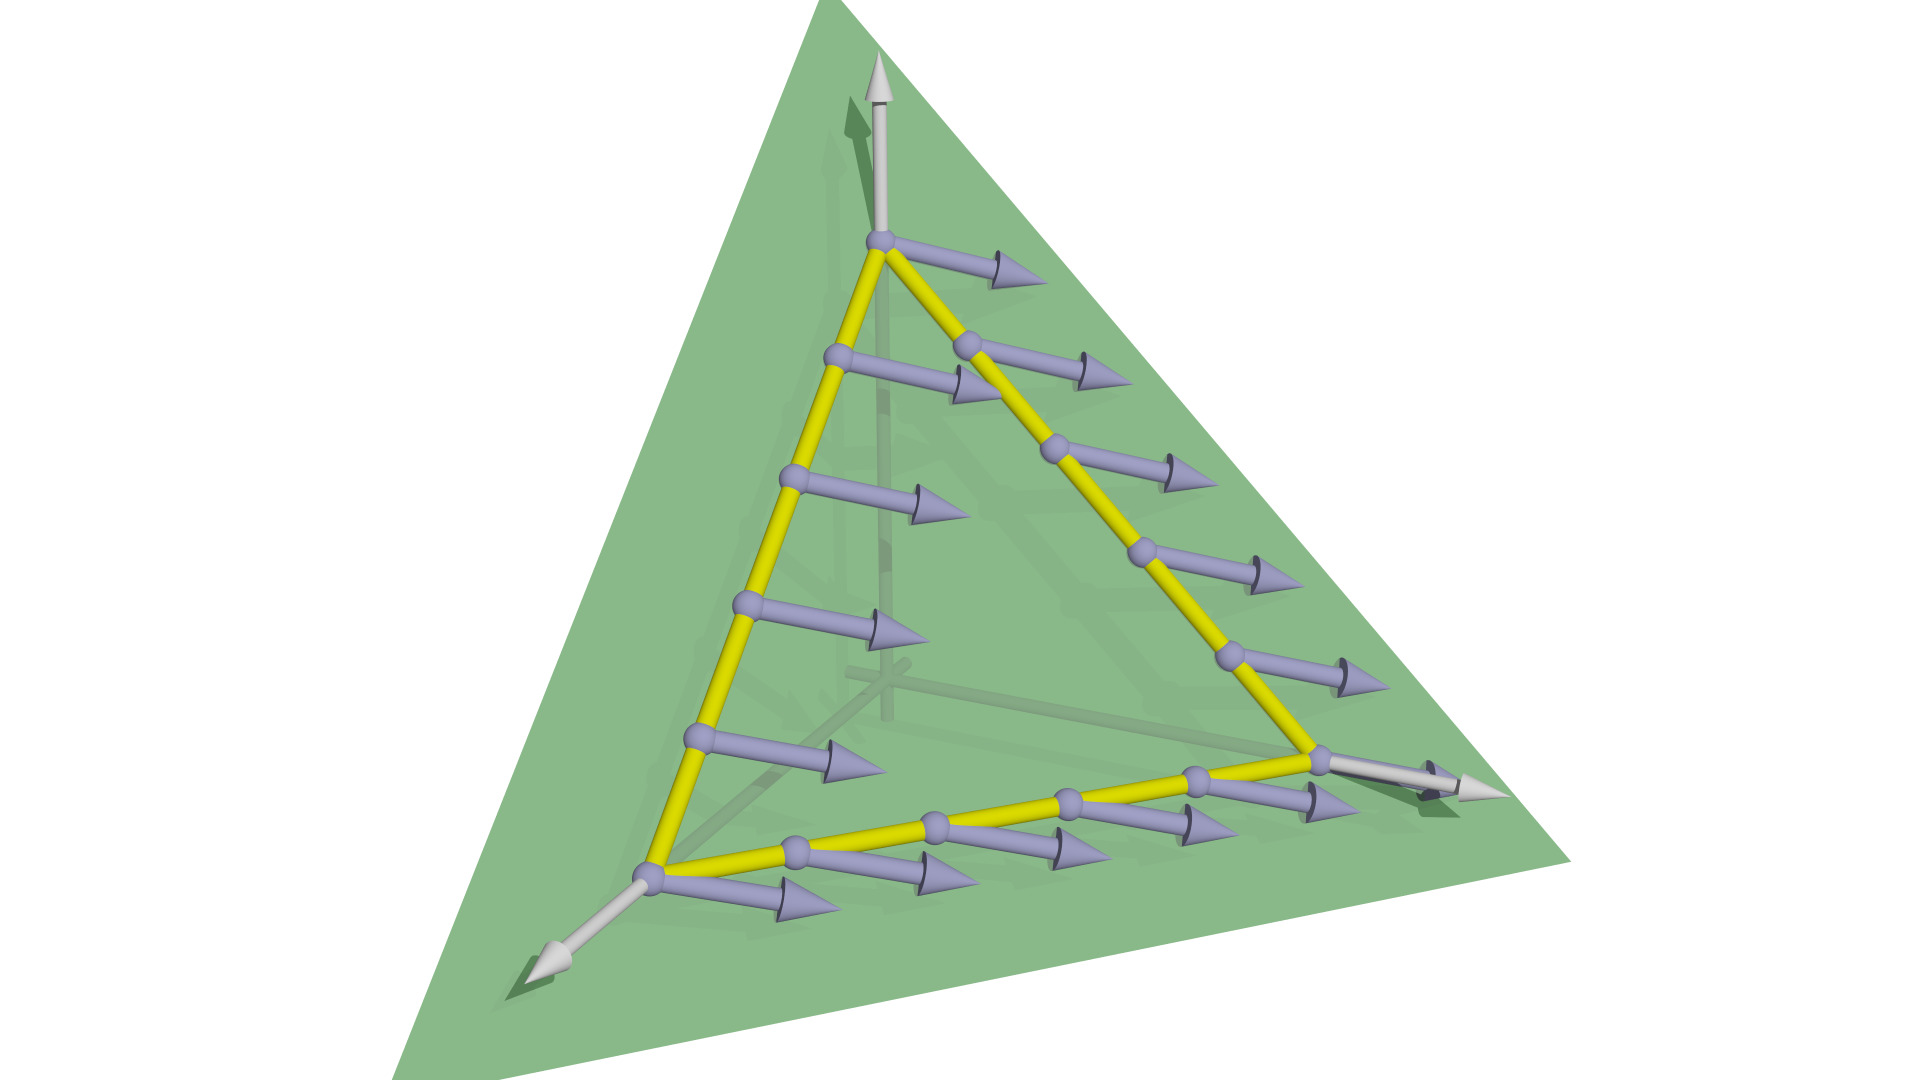
\includegraphics[width=\hsize]{chapters/3d/flach.jpg}
\caption{Beim Paralleltransport eines Vektors entlang einer Kurve in
einer Ebene dreht sich der Vektor nicht
\label{skript:kruemmung:transportflach}}
\end{figure}
\begin{figure}
\centering
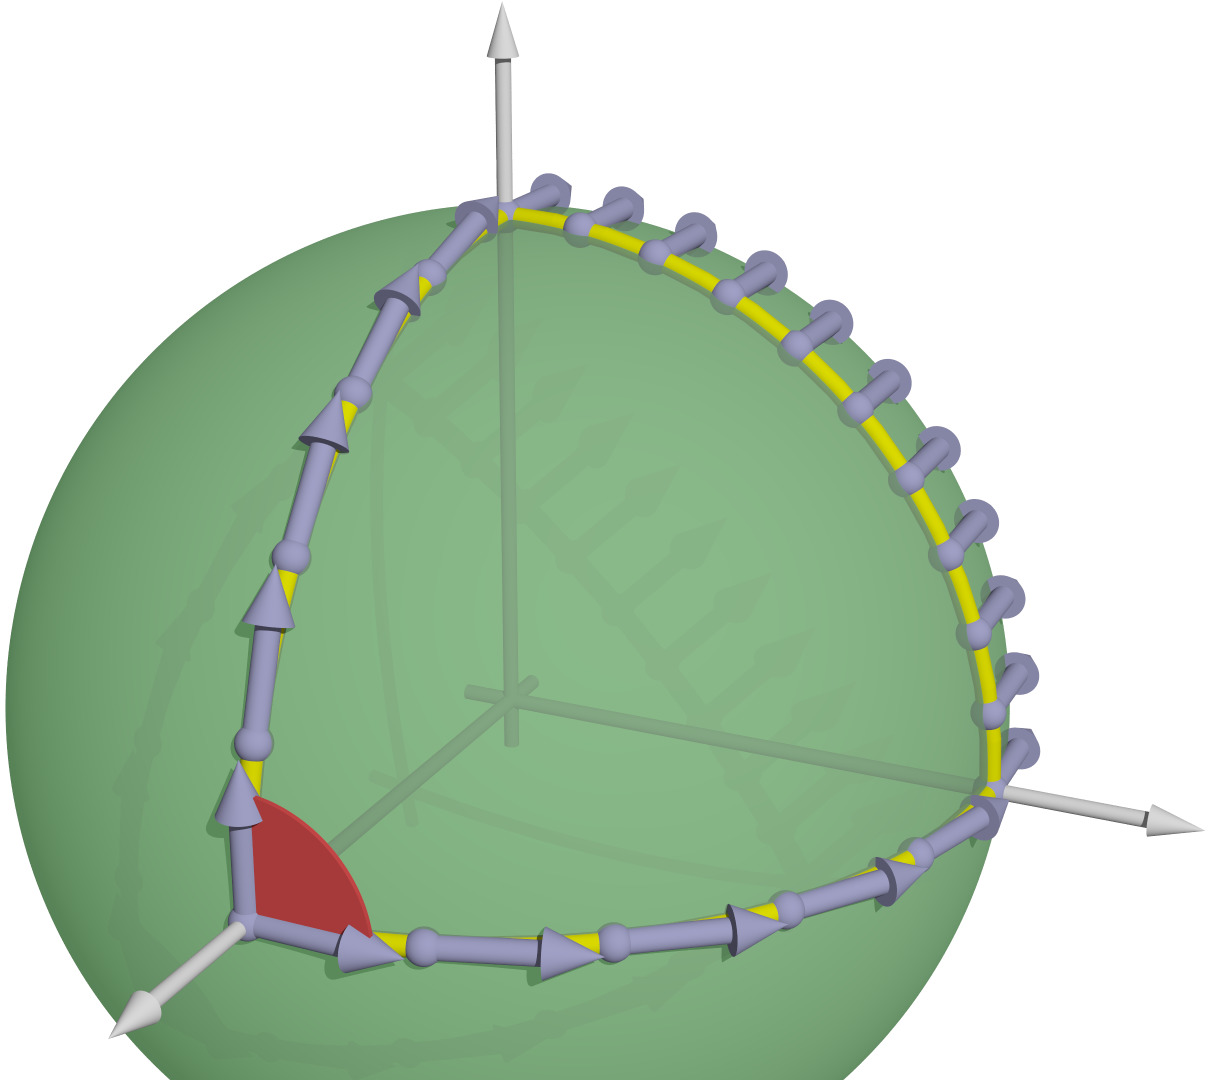
\includegraphics[width=\hsize]{chapters/3d/sphere.jpg}
\caption{Drehung eines Tangentialvektors beim Transport entlang eines
Dreiecks auf der Kugeloberfläche.
Der Flächeninhalt des Dreiecks ist ein Achtel der Kugeloberfläche,
also $4\pi/8=\pi/2$, der Drehwinkel ist $\pi/2$.
\label{skript:kruemmung:transportkugel}}
\end{figure}

Transportiert man einen Vektor in der Ebene mit dem üblichen euklidischen
Koordinatensysteme parallel, dann ändert seine Richtung nicht,
denn die Christoffelsymbole verschwinden alle
(Abbildung~\ref{skript:kruemmung:transportflach}).
Auf einer Kugeloberfläche sieht das ganz anders aus.
Transportiert man einen Vektor tangential an den Äquator zunächst entlang 
des Äquators über einen Winkel von $90^\circ$, dann auf einem Längenkreis
bis zum Nordpol und wieder zurück zum Ausgangspunkt.
Wie in Abbildung~\ref{skript:kruemmung:transportkugel}
sichtbar, dreht sich der Vektor
dabei um $90^\circ$. 
Der Unterschied rührt natürlich daher, dass die Kugeloberfläche gekrümmt
ist.
Offenbar ist die Änderung der Richtung eines Tangentialvektors beim
Paralleltransport entlang eines geschlossenen Weges ein Mass für die
Krümmung einer Fläche.

In diesem Kapitel wollen wir zeigen, wie aus dem Konzept des
Paralleltransportes ein mathematisch wohldefiniertes Mass für die
Krümmung gewonnen werden kann.

\subsection{Krümmungstensor}
Wir möchten Berechnen, wie sich ein Vektor beim Paralleltransport entlang
einer geschlossenen Kurve ändert.
In dieser Form ist das Problem sicher zu kompliziert, die Wahl
einer geschlossenen Kurve beinhaltet viel zu viele Freiheitsgrade.

Zu zwei Tangentialvektoren $u^\mu$ und $v^\mu$ und in einem Punkt
$P$ können wir immer eine
Fläche finden, die aus Geodäten besteht, die alle vom Punkt $P$ ausgehen
und dort eine Richtung haben, die eine Linearkombination der beiden
Tangentialvektoren ist.
Mit diesem Trick können wir das Problem auf eine zweidimensionale
Fläche reduzieren.
Und statt eine beliebige Kurve zuzulassen, können wir uns weiter
auf einen Polygonzug beschränken, bei dem wir den Geodäten folgen,
die als Tangentialrichtung die Richtung der beiden gegebenen
Tangentialvektoren haben.

Wenn wir einen Vektor $x^\mu$ entlang einer solchen Kurve parallel
transportieren, dann aber die Kurve auf einen Punkt zusammenschrumpfen
lassen, dann entsteht im Grenzwert ein Vektor $y^\mu$,
der die Verschiebung des Vektors $x^\mu$ beschreibt.
Dieser Vektor muss linear von $u^\mu$, $v^\mu$ und $x^\mu$ abhängen,
wir erwarten also, dass in jedem Punkt Zahlen
$R^\alpha\mathstrut_{\mu\nu\sigma}$ geben muss, mit denen man
$y^\mu$ berechnen kann:
\[
y^\alpha = R^\alpha\mathstrut_{\mu\nu\sigma}u^\mu v^\nu x^\sigma.
\]

\subsection{Ricci-Krümmung}

